\subsection{M\'exico}\label{subsec:mex}

\subsubsection*{Detector description}

Sierra Negra is the first LAGO site with WCD working (since early 2007). Until
2010, 3$\times$4\,m$^{2}$ area Cherenkov detectors, in a 30\,m triangular array
were taking data at this site each detector had an EMI 9030A photomultiplier
tube, looking towards the bottom. The output of the phototube was connected to
a data acquisition card used in the development of this phase.

\subsection*{Upgrade of the SN LAGO set up}

The Sierra Negra site of the LAGO experiment has four detector of 40\,m$^{2}$,
three of them located at the vertex of an equilateral triangle of 30\,m. 
Those detectors are cylindrical tanks, made with a corrugated steel plated
bolted with stainless steel screws, 7.3\,m of diameter and 1.15\,m high. The
tops and inside of each detector are covered by an EPDM (Ethylene Propylene
Diene Monomer) black liner to contain and protect the radiator media.
The EPDM material is elastic, easy to weld and mechanically very strong,
helping to have a light tight and insulated inner environment. The body and
the bottom of the detector are covered with a bag of high diffusive and
reflective material: white polyethylene banner. The white bag is filled with
high quality purified water up to a level of 1.1\,m and in the upper surface;
there is a Tyvek sheet floating in order to reflect the Cherenkov light
produced as uniformly as possible. The special feature of this kind of Water
Cherenkov Detector is its inner segmentation. To improve the light collection,
we have installed reflective walls with the same material that the inner liner,
The cylinder was divided at four regular sectors; one hemispherical 8" diameter
PMT located in the centroid of each one, looking downwards, The PMT
photocathode is submerged to avoid losses by any air-water interface. The
entire container is covered and protected externally by a black, light-tight
bag and a canvas roof. The Cherenkov light is collected by the electron
phototube 9354KB of Electron Tubes Ltd., installed up towards the bottom.

\begin{figure}[th!]
\centering
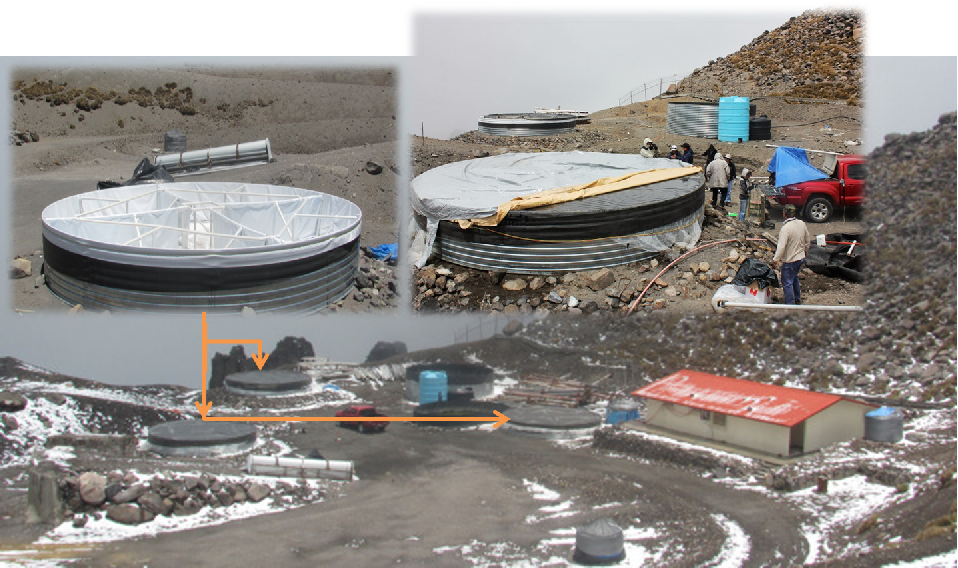
\includegraphics[width=0.8\textwidth]{images/mexico/sitelago-01.png}
\caption{LAGO Sierra Negra WCDs. An old array of small tanks is clearly seen
between the new big stainless steel tanks.  Those are covered by a black EPDM
liner. B.- Internal structure of the new WCD. The structure of the PVC pipes
allows us to set the banner walls to divide it into four sectors and fix the
PMT and cables in a safety way. Also help us to keep 
the upper liner and a canvas roof.}
\label{sitelago01}
\end{figure} 

At the center of the array we will set a WCD with the same area, but 4.5\,m height, 
filled with clean water and 4 PMT at the bottom looking upwards. This detector
has the aim to reject hadrons when a extensive air shower is detected.

\subsection*{Operation and calibration of the WCD Detectors}

Calibration mode. It consists on the data acquisition of 32 consecutive samples
in 10 ns intervals (100\,MSPS\footnote{Mega Samples Per Second}) of the digital
pulses produced by an ultraviolet LED with wavelength of 405\,nm with a 15\,ns
wide pulse in a frequency of 10\,kHz located 60\,cm from the PMT. The phototube
polarization voltage and the LED polarization voltage are fine tuned. It
provides us with a minimal response that represents a fundamental part for the
calibration of a PMT.

As shown in figure \ref{sitelago04} and figure, \ref{sitelago05}, we can plot
the response to a single photo-electron using our DAQ (see section
\ref{sec:detector}). The curves correspond to high voltages of 1.25\,kV,
1.3\,kV, and 1.35\,kV. The best single photo-electron response, for this PMT,
is obtained at 1.3\,kV and this value was set as the operation one.

\begin{figure}[t]
\centering
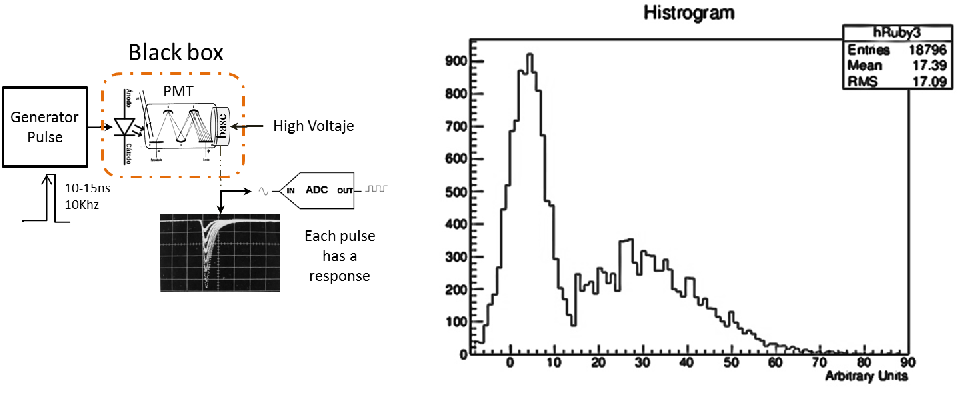
\includegraphics[scale=0.4]{images/mexico/sitelago-04.png}
\caption{Mode calibration and Response to a single photo-electron, using the new DAQ.}
\label{sitelago04}
\end{figure} 

\begin{figure}[t]
\centering
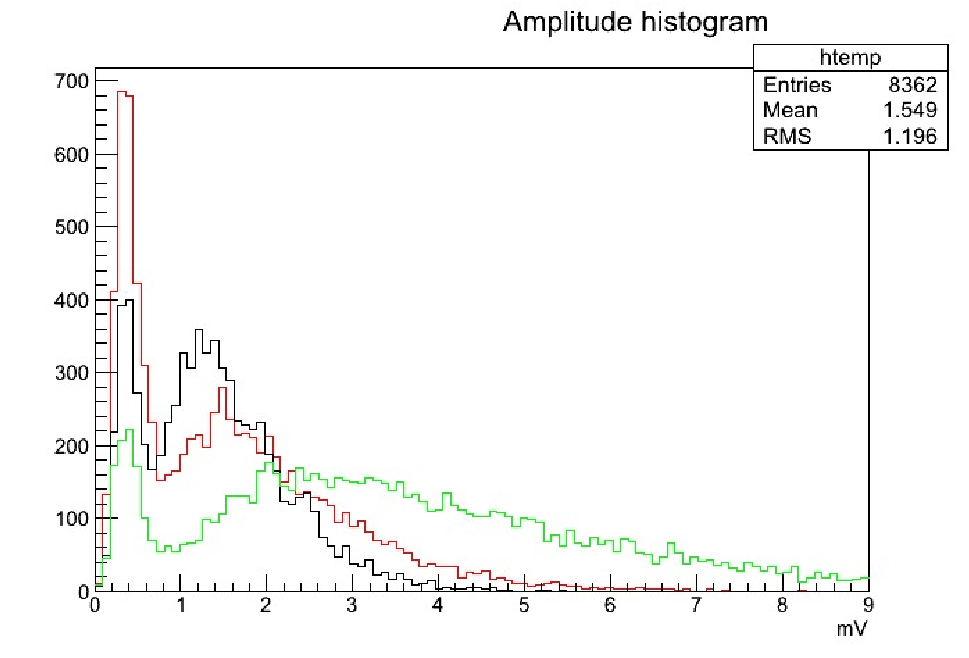
\includegraphics[scale=0.4]{images/mexico/sitelago-05.png}
\caption{Plot of the response to a single photo-electron by the PMT at 1.25\,kV (black), 1.3\,kV (red), and 1.35\,kV (green). The operation voltage was fixed at 1.3\,kV.}
\label{sitelago05}
\end{figure} 

%Examples of traces, baseline and threshold are shown in \ref{sitelago06}.
%
%\begin{figure}[t]
%\centering
%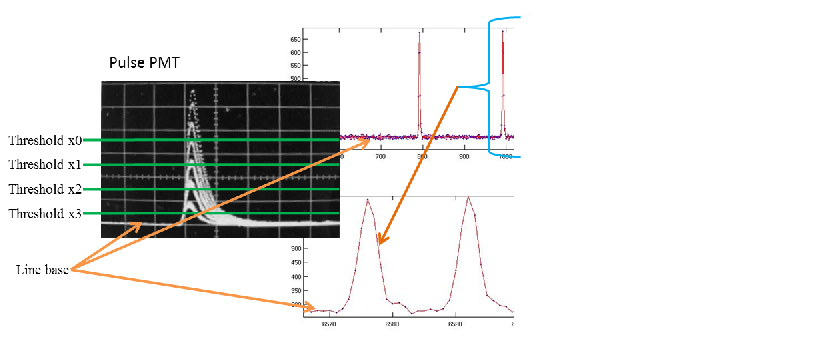
\includegraphics[scale=0.5]{images/mexico/sitelago-06.png}
%\caption{Example who shows the base line the trace and the rate.}
%\label{sitelago06}
%\end{figure} 
